\documentclass[12pt, a4paper, notitlepage]{report}
\usepackage{mathptmx}
\usepackage[T1]{fontenc}
\usepackage[utf8x]{inputenc}
\usepackage[english]{babel}
\usepackage{graphicx}
\usepackage{float}
\usepackage{amsmath}
\usepackage{mathtools}
\usepackage{amsfonts}
\usepackage{enumerate}
\usepackage[caption = false]{subfig}
\usepackage[top=2.5cm, bottom=2.5cm, left=2cm, right=2cm]{geometry}
\usepackage[font={small,it}]{caption}
\usepackage{fancyhdr}
\usepackage{listings}
\usepackage{color}

\definecolor{dkgreen}{rgb}{0,0.6,0}
\definecolor{gray}{rgb}{0.5,0.5,0.5}
\definecolor{mauve}{rgb}{0.58,0,0.82}
\definecolor{lyellow}{rgb}{1,1,0.9}

\lstset{backgroundcolor=\color{lyellow},
	frame=tb,
	language=Python,
	aboveskip=3mm,
	belowskip=3mm,
	showstringspaces=false,
	columns=flexible,
	basicstyle={\small\ttfamily},
	numbers=none,
	numberstyle=\tiny\color{gray},
	keywordstyle=\color{blue},
	commentstyle=\color{dkgreen},
	stringstyle=\color{mauve},
	breaklines=true,
	breakatwhitespace=true,
	tabsize=3
}

\pagestyle{fancy}
\lhead{Tommaso Tabarelli}
\chead{\thepage}
\rhead{\today}
\cfoot{Information theory and computation}
\rfoot{A.y. 2019/2020}
\lfoot{Exercise 3}

\begin{document}

\begin{center}
	\LARGE{Quantum information and computation: homework 4}\\
	\Large{of Tommaso Tabarelli}
\end{center}


\begin{abstract}
	In this homework we are asked to do a deeper analysis of previous exercises results. We are asked to make automatic data generation, plot and fit using a python script. Its aim is to modify an input file with stored matrix dimensions and to call a fortran script that reads it and measures computation performance. After this, python script also takes care of calling Gnuplot to plot and fit results, eventually collecting the results.
\end{abstract}

\section*{Theory}
Scripting is used when there are some operations that have to be called many times on different objects: instead of make similar calls manually (that can take a long time, being boring and not error-free) a script is usually prepared to make several calls to programs or comands. This way, a single call to the script can be performed, avoiding time losses and human errors.

\section*{Code development}
In first python script libraries to interface with the operative system are imported. My script can read minimum and maximum matrix dimension and step size to move from former to latter from the command line, creating the corresponding list. After this, it checks for old files and eventually deletes them: this is done to keep fortran code as simple as possible because it is easier to handle file using python with respect to fortran.\\
At this point the proper task is performed: python script enters a loop in which matrix dimensions are written to a file and fortran executable is called. Fortran program reads dimensions from the file, initializes two square matrices with random real numbers and finally performs matrix multiplication in three different ways measuring execution time for each. Time results is then written into other files, one different file for every different way to evaluate matrix multiplication.\\
A second python script takes care of collecting results calling a gnuplot script which performs a quadratic and a cubic fit for every method and plots coefficients in othes files.\\
Another gnuplot script takes care of plotting the whole results in a single plot to compare the different methods.\\

\begin{lstlisting}
#!/usr/bin/python

import os
import subprocess as sub
import sys
import numpy as np

N_min = int(sys.argv[1])
N_max = int(sys.argv[2])
Step = int(sys.argv[3])

# Checking reasonable dimensions
if (N_min<=0 or N_max<=0):
	print("\n\tN_min/N_max souhld be greater than 0...\n\tStopping program.\n")
	sys.exit()

# Checking N_min <= N_max
if (N_min>N_max):
	print("\n\tN_min sould be smaller than N_max...\n\tStopping program.\n")
	sys.exit()

# Creating a logarithmic spacing (it spans more magnitudes than linear spacing)
# dim_list = np.logspace( np.log10(N_min), np.log10(N_max), 10, dtype=np.int16)
dim_list = np.arange( N_min, N_max, Step, dtype=np.int16)

# Cleaning old files
file_list = ["results_m.txt", "results_T.txt", "results_F.txt"]

for filename in file_list:
	if os.path.isfile(filename):
		os.remove(filename)

# Executing task
for ii in dim_list:
	ofile = open("dim_file.txt", "w+")
	ofile.write(str(ii))
	ofile.close()
	sub.run(["./Ex4_Tommaso_Tabarelli_CODE.exe"])
\end{lstlisting}

\begin{lstlisting}
#!/usr/bin/python

import os
import subprocess as sub
import sys
import numpy as np

file_list = ["results_m.txt", "results_T.txt", "results_F.txt"]
existing_files = []
labels = []

path = os.getcwd()
temp_name = path+"/results.txt"

for filename in file_list:
	if os.path.isfile(filename):
	existing_files.append(filename)
	# Creating a label for every different file
	labels.append(filename[filename.find(".txt")-2:filename.find(".txt")])
	
	# Executing task
	for file_,label in zip(existing_files,labels):
	
	file_ = path+"/results_m.txt"
	# Renaming file to use Gnuplot script
	sub.run(str("mv "+file_+" "+temp_name), shell=True)
	os.system(str('gnuplot "Gnu_fit.gnu"'))
	
	# Resetting original name
	sub.run(str("mv "+temp_name+" "+file_), shell=True)
	
	# Renaming files created by Gnuplot
	sub.run(str("mv "+path+"/fit_time_dim.log "+path+"/fit_time_dim"+label+".log"), shell=True)
	sub.run(str("mv "+path+"/quadratic_fit_coef.txt "+path+"/quadratic_fit_coef"+label+".txt"), shell=True)
	sub.run(str("mv "+path+"/cubic_fit_coef.txt "+path+"/cubic_fit_coef"+label+".txt"), shell=True)
	sub.run(str("mv "+path+"/Fit.png "+path+"/Fit"+label+".png"), shell=True)

os.system(str('gnuplot "plot_res.gnu"'))
\end{lstlisting}


\section*{Results}
The program runs well with no errors. The execution of the script generates the following images.

\begin{figure}[H]
	\centering
	{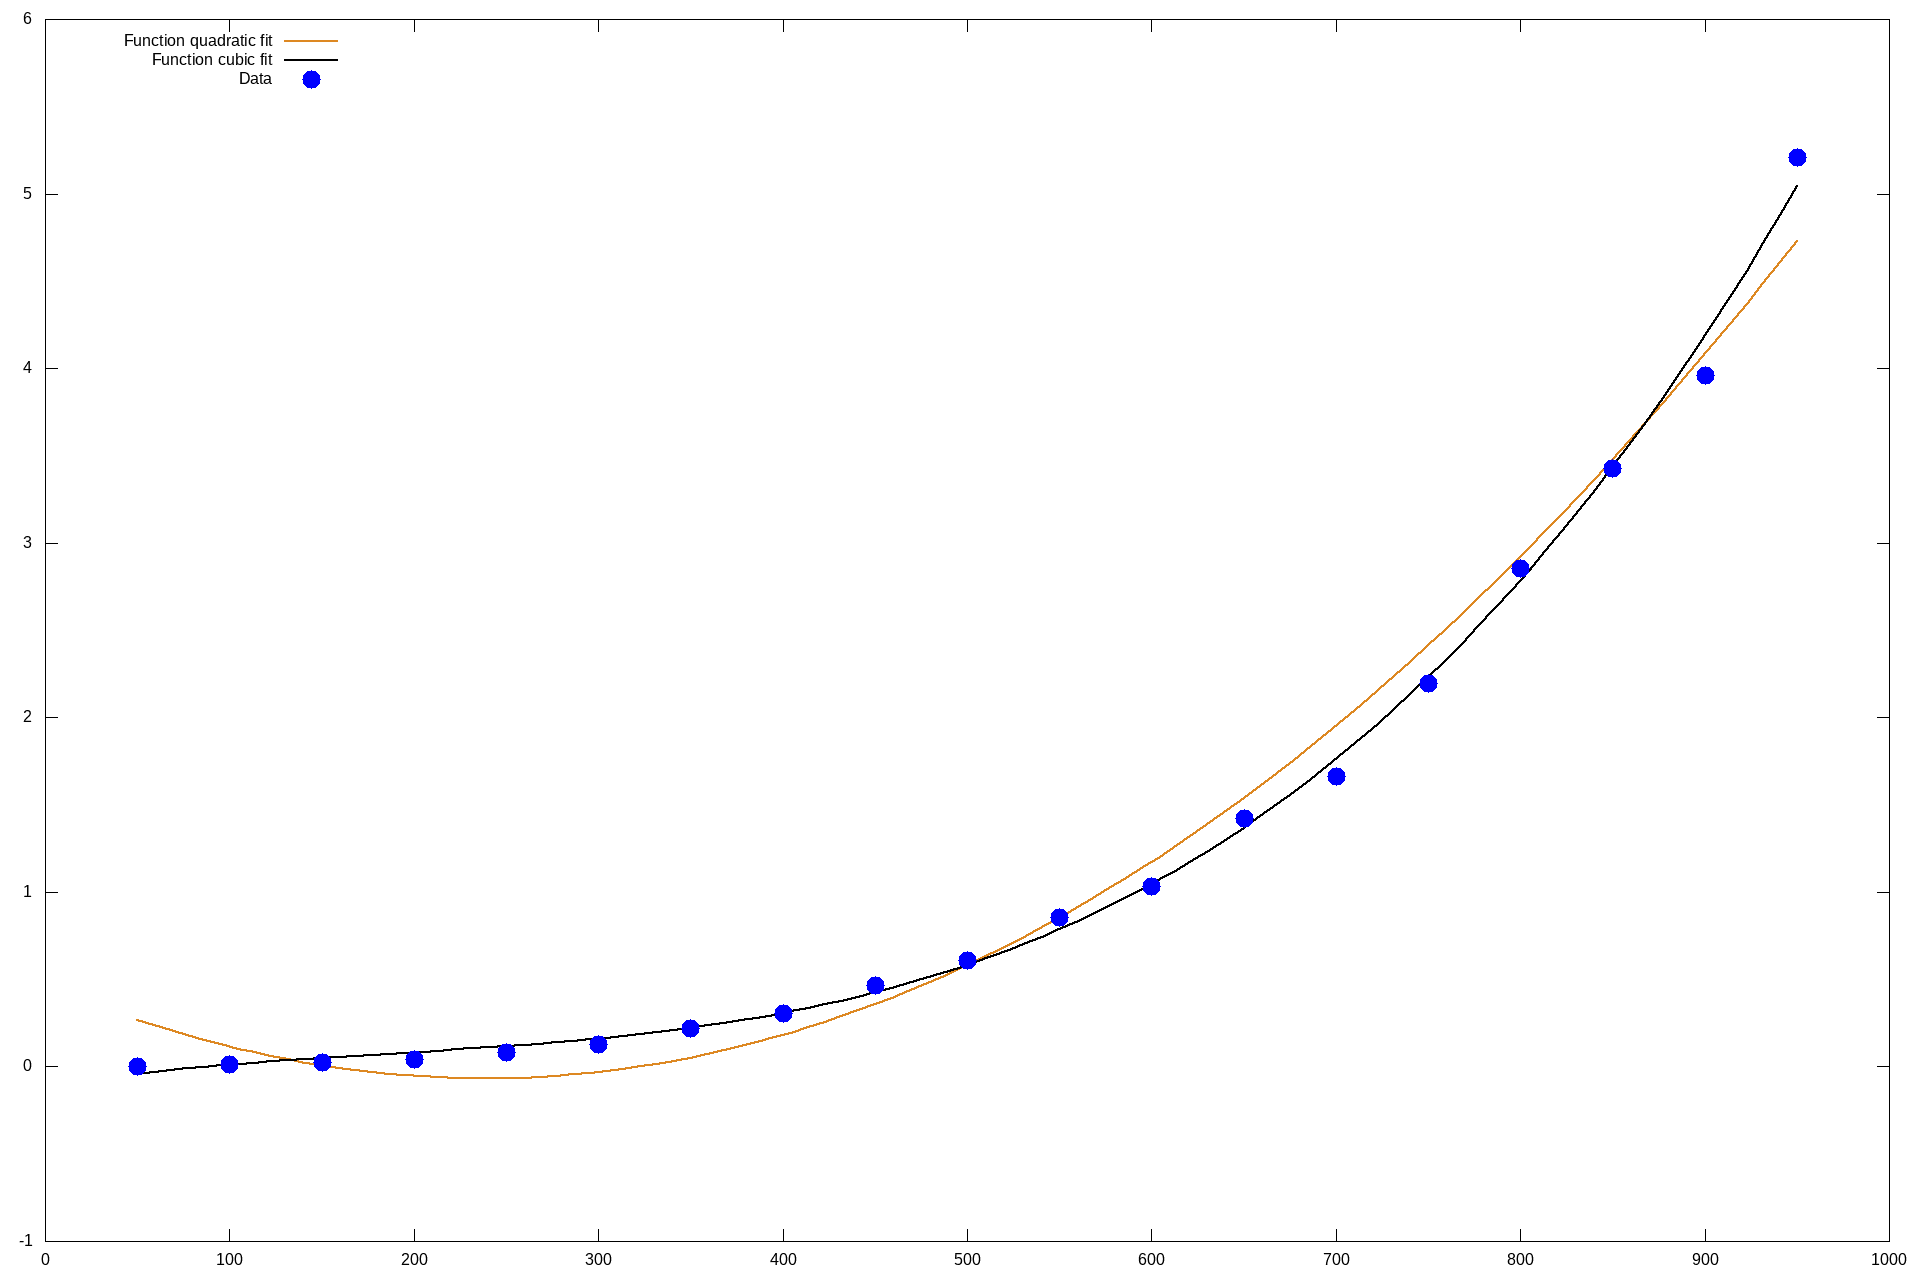
\includegraphics[scale=0.3]{Fit_m.png}} 
	\caption{Results for manual method.}
	\label{figure_lambdas}
\end{figure}

\begin{figure}[H]
	\centering
	{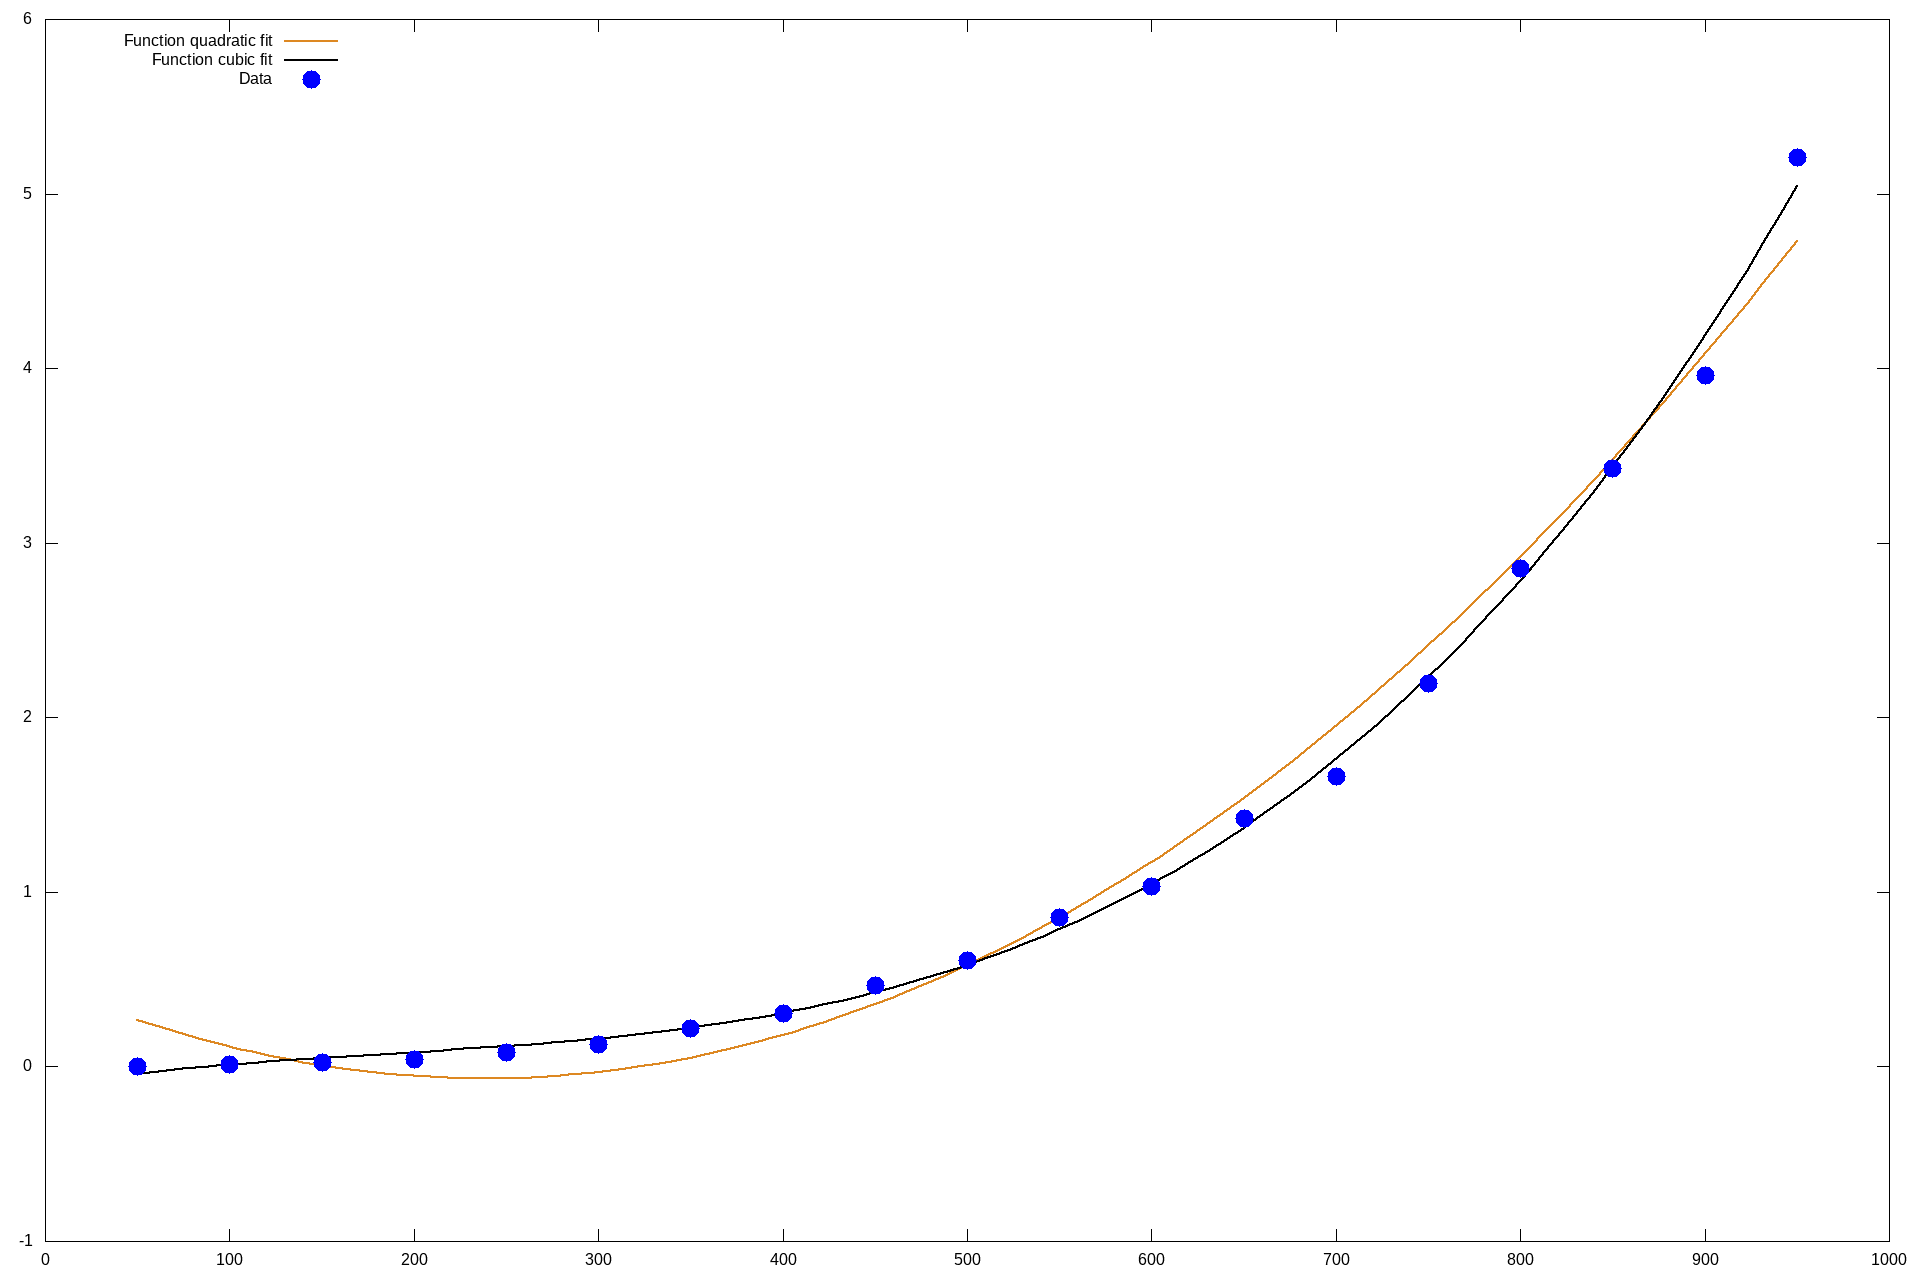
\includegraphics[scale=0.3]{Fit_T.png}} 
	\caption{Results for manual transposed method.}
	\label{figure_lambdas}
\end{figure}

\begin{figure}[H]
	\centering
	{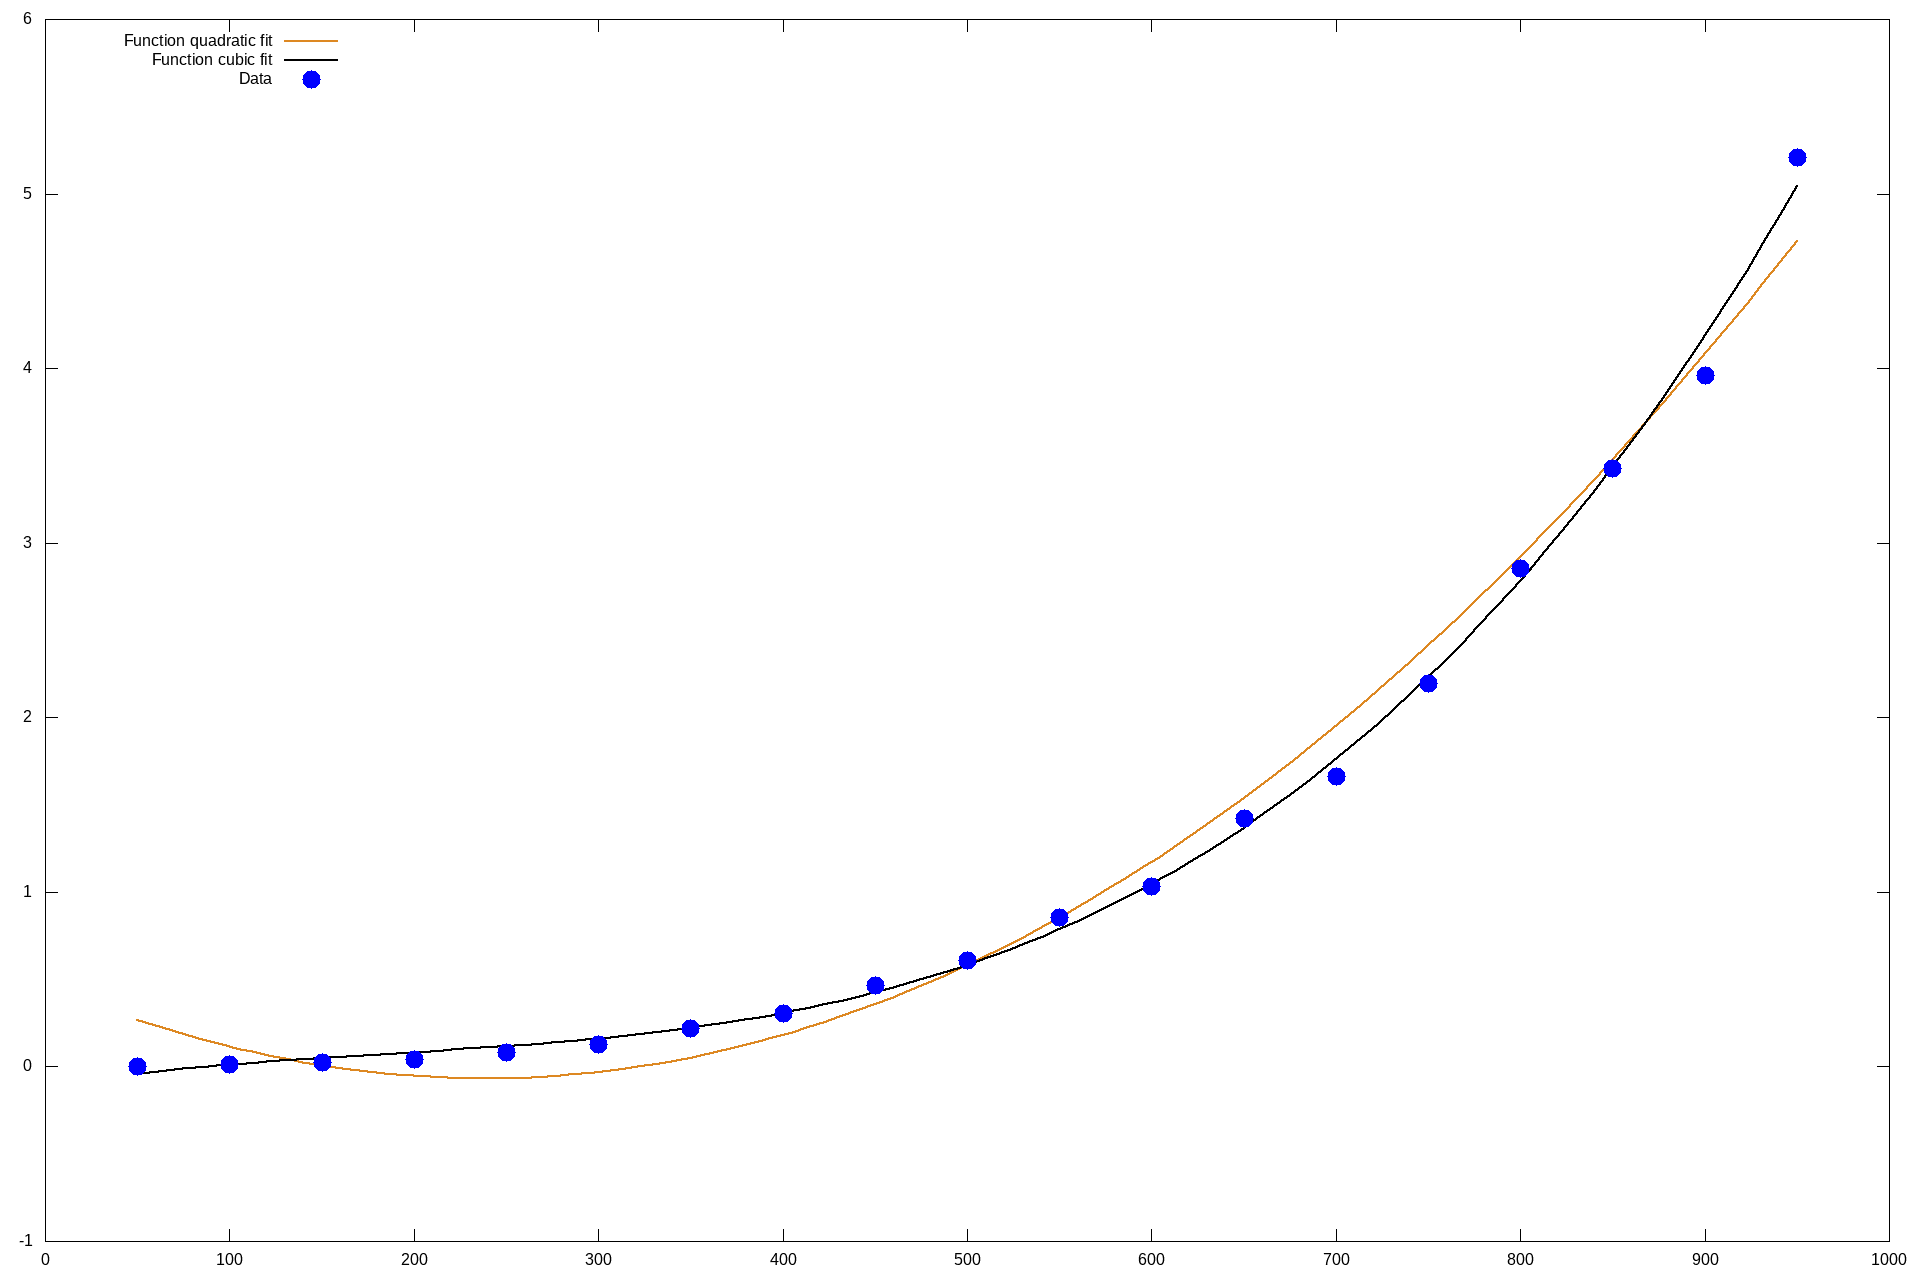
\includegraphics[scale=0.3]{Fit_F.png}} 
	\caption{Results for matmul method.}
	\label{figure_lambdas}
\end{figure}

\begin{figure}[H]
	\centering
	{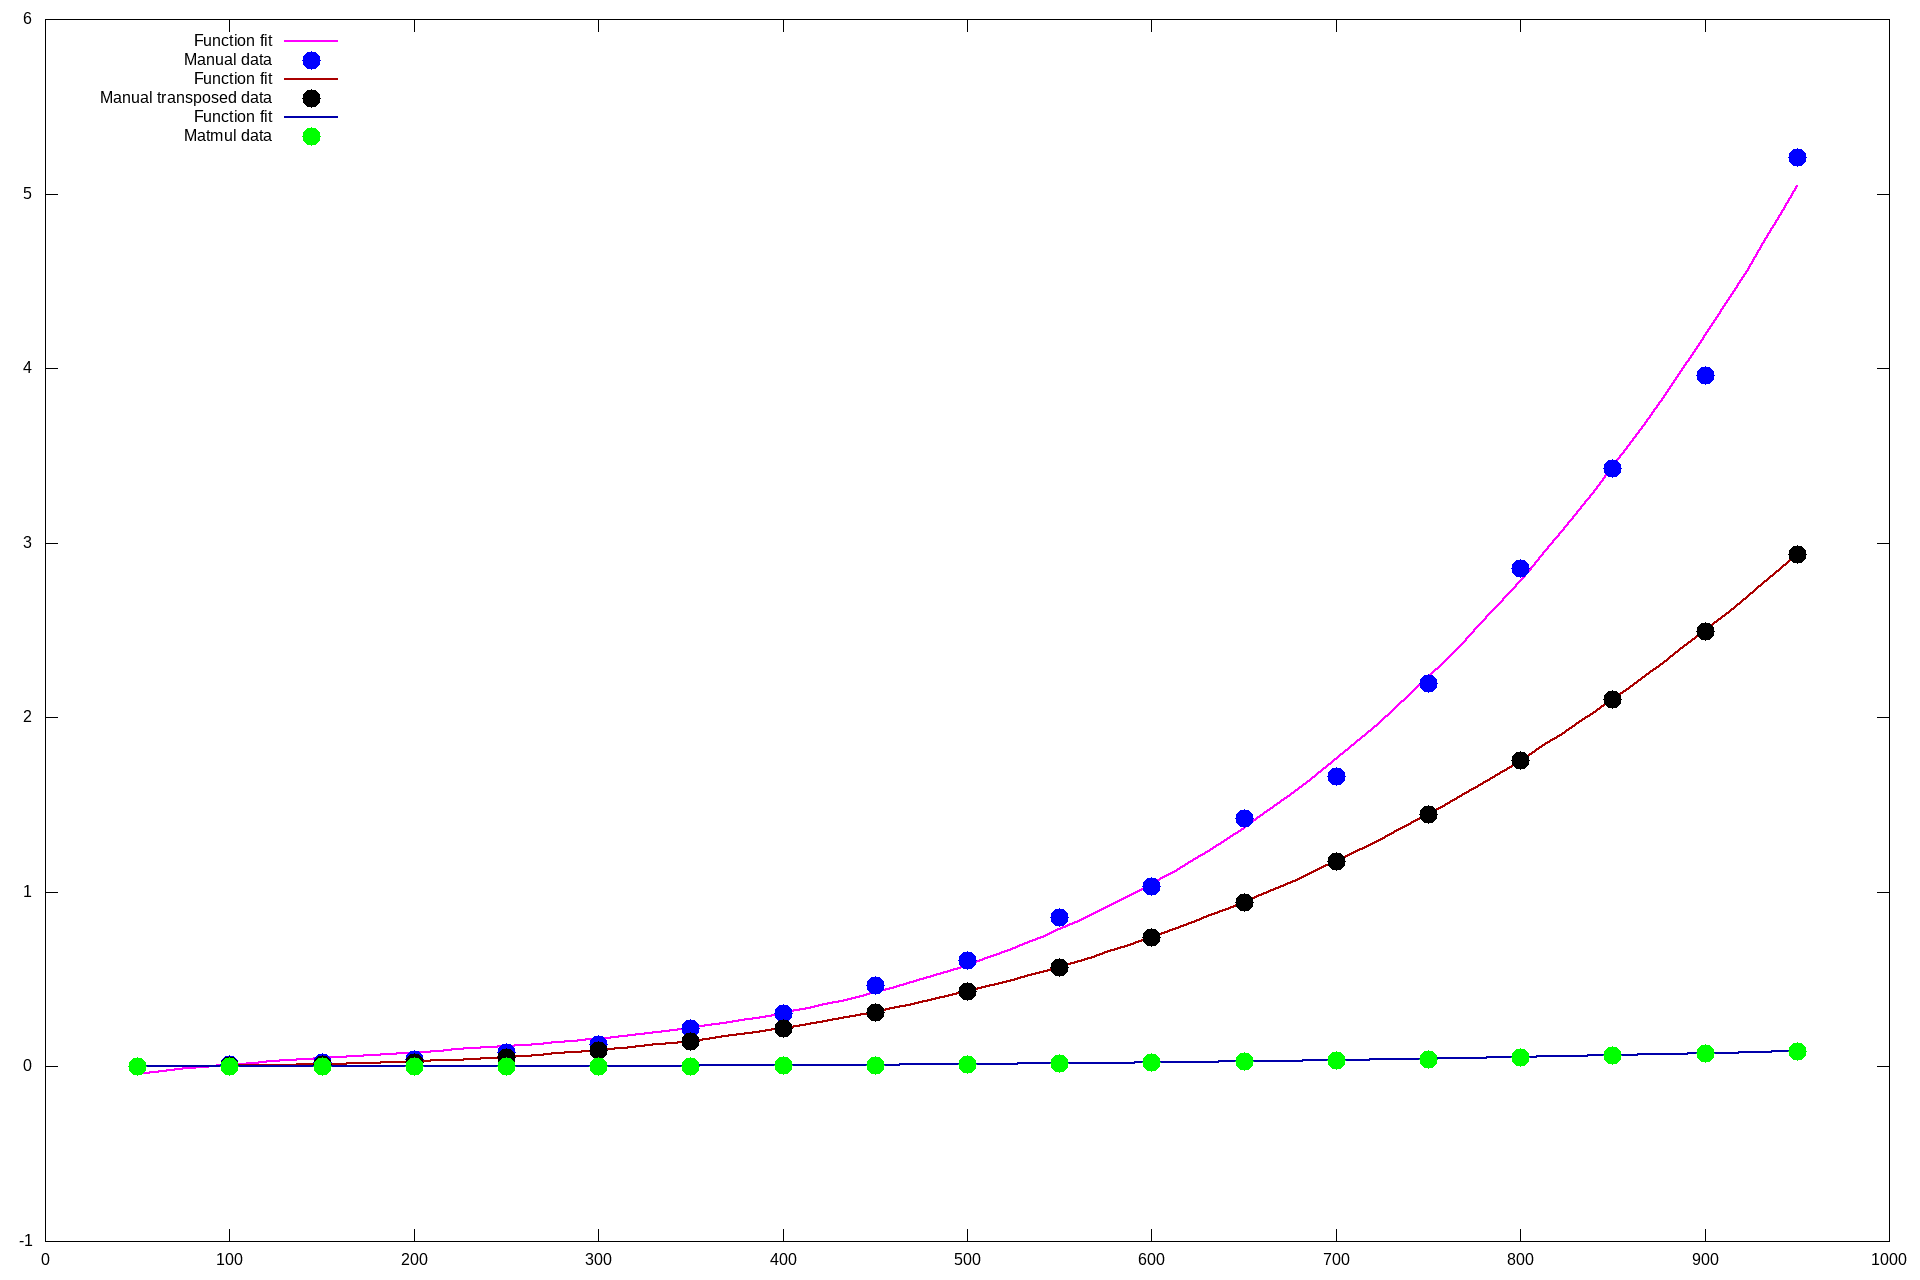
\includegraphics[scale=0.3]{Fit_comp.png}} 
	\caption{Comparison between results.}
	\label{figure_lambdas}
\end{figure}

The results are slightly better for matmul computation.\\
Cubic function seems to fit better the results.

\section*{Self-evaluation}
During this exercise I learned how to implement a python scripts that deals with system calls.\\
To improve this script it can be changed to ask more parameters as input.\\
File names can be extended to contain more runtime parameters in them to better save results and retrieve them when necessary.
\end{document}